\documentclass[11pt]{article}
\usepackage[T1]{fontenc}
\usepackage[utf8]{inputenc}
\usepackage[margin=1in]{geometry}
\usepackage{amsmath,amssymb,booktabs,graphicx,hyperref,array}
\setlength{\emergencystretch}{2em}
\hypersetup{colorlinks=true,linkcolor=blue,citecolor=blue,urlcolor=blue}
\title{A Dose-Dependent Crossover in Transcoder Fidelity:\\Beating Local Linearization Is Not Finite-Effect Accuracy}
\author{Author information to be supplied}
\date{November 4, 2026 --- private working manuscript, version 16}
\begin{document}
\maketitle
\begin{abstract}
A public transcoder can be a poor local model of a native MLP and still predict the downstream effect of a large intervention accurately. On 256 fresh name-pair blocks, a fixed Gemma-3-270M layer-15 transcoder predicts the pronoun-readout effect of a full donor patch with 10.11\% relative RMS error, versus 129.96\% for native-vector Taylor and 28.05\% for a FIT-trained ridge map. At dose .05 the ranking reverses: 117.46\% for the transcoder, 12.10\% for Taylor. The large-dose advantage persists for projected edits that do not reach the donor state, at twice the donor difference, and on a held-out template. A second public artifact, Gemma-3-1B layer 22, repeats the Taylor--transcoder crossover but not the accuracy: at the full patch it loses to zero change and to ridge. Outperforming local linearization is therefore not evidence of finite-effect fidelity; the relevant test is dose-resolved accuracy against strong baselines. We further characterize the first artifact's errors through endpoint cancellation and a small set of decisive threshold switches, and report a negative boundary for a Qwen cross-layer transcoder component.
\end{abstract}

\section{Introduction}
Transcoders and cross-layer transcoders are increasingly used as replacement models: to read circuits, to choose features to steer, and to predict what an edit will do. Their fidelity is usually judged locally, through reconstruction or Jacobians~\cite{shabalin2026}, while the use cases involve finite interventions. These two regimes need not agree. First-order approximations are known to break down at large intervention strengths~\cite{syed2023,guo2026}, but how a sparse replacement behaves across that range, relative to the native model's own linearization, has not been measured.

We measure it. For a fixed public transcoder we sweep the intervention dose from a small fraction of a donor difference to twice the full patch, propagate every prediction through the exact native downstream network, and score the predicted change of a two-token readout. On Gemma-3-270M layer 15 we find a clean crossover: native Taylor is far better at small dose, the transcoder far better at the full patch, where it also beats a ridge map trained on native vector changes. The result holds on a fresh lexical TEST frozen in advance, on a held-out template, for projected edits and at dose 2.

The second finding qualifies the first. On Gemma-3-1B layer 22, the same crossover appears, yet the transcoder's full-patch error exceeds that of predicting no change. Beating Taylor at large dose is therefore a weak criterion: Taylor itself is poor there. Useful finite-effect accuracy is a separate, measurable property, and the two artifacts differ in it.

Diagnostics on the first artifact then ask what its favorable error looks like. Endpoint reconstruction errors largely cancel in the predicted difference, and removing the threshold switches of 32 FIT-selected features destroys the full-patch accuracy, while keeping only them preserves it. A Qwen3-0.6B cross-layer transcoder component, finally, stays at the zero-change baseline across all doses. Table~\ref{tab:scope} maps the cohorts; the supplement holds the complete earlier record.

\begin{table}[ht]\centering\scriptsize
\setlength{\tabcolsep}{4pt}
\begin{tabular}{>{\raggedright\arraybackslash}p{.20\textwidth}>{\raggedright\arraybackslash}p{.34\textwidth}>{\raggedright\arraybackslash}p{.37\textwidth}}\toprule
Study & Sample and reuse & Reporting scope\\\midrule
Gemma-270M main & 256 fresh name-pair blocks; so/when and transfer share names; 1,536 contexts & Fixed six-dose/two-operator TEST; qualified intervals for 12 full-dose TC metrics.\\[3pt]
Gemma-1B replication & 256 additional disjoint blocks; six doses, full donor operator & Frozen FIT/protocol; nominal block intervals.\\[3pt]
Residual/mask tests & 32 previously observed 270M blocks; 768 conditions & Posthoc oracle and mask diagnostics.\\[3pt]
Fixed-norm directions & Cached FIT32; observed TEST32; fresh 32 blocks & Descriptive; transfer 45/64 and object 12/64 contexts eligible.\\[3pt]
Qwen boundary & 256 blocks shared with the companion study & Descriptive CLT-component dose curve.\\\bottomrule
\end{tabular}
\caption{Evidence map. Lexical blocks are the sampling units; templates, doses and control groups are dependent measurements within blocks.}\label{tab:scope}
\end{table}

\section{Related work}
Transcoder circuits and their validation are established~\cite{dunefsky2024,ameisen2025}. Shabalin and Piotrowski~\cite{shabalin2026} compare transcoder and native Jacobians and explicitly restrict themselves to first-order faithfulness rather than faithfulness under interventions; formal discrepancy bounds~\cite{ladner2026} cover activation sets rather than intervention effects. That gap is the subject of this paper. Jacobian sparse autoencoders~\cite{farnik2025} sparsify computation rather than test a replacement's finite response, and JumpReLU thresholds~\cite{rajamanoharan2024} make discontinuous responses expected.

On the linearization side, attribution patching is known to degrade with intervention size~\cite{syed2023,zhangwang2026}. Guo et al.~\cite{guo2026} show that first-order intervention attribution tracks ablation effects at moderate steering scales and breaks down at several times larger scales; they do not compare a sparse surrogate against the gradient at large scale. Our Taylor comparator linearizes only the branch vector and keeps the exact nonlinear suffix, so its large-dose failure is not a scalar first-order artifact. Bazán Sánchez~\cite{bazan2026} predicts full feature removal from a measured midpoint inside replacement models; our predictions use no measured intermediate effect and are scored against native interventions. Strength controls change sparse-code comparisons~\cite{zhang2026}, and matched-effect evaluation~\cite{luo2026} motivates our explicit statement of what fixed-norm controls do and do not equalize. Deshpande~\cite{deshpande2026} asks which readouts survive sparse compression, a complementary question about readouts rather than intervention deltas.

\section{Prediction target and experimental design}
\subsection{Native changes and downstream readout}
Let $f(z)$ be the native branch, including its documented normalization, and $T(z)$ the fixed transcoder. Recipient input $z$, donor difference $d=z_d-z$ and a unit FIT class-mean direction $w$ define
\[
 \delta_{full}=cd,\qquad \delta_{proj}=c(d^\top w)w,
 \quad c\in\{.05,.1,.25,.5,1,2\}.
\]
The native target and main predictions are
\[
 \Delta_N=f(z+\delta)-f(z),\quad
 \Delta_T=T(z+\delta)-T(z),\quad
 \Delta_J=J_f(z)\delta.
\]
Each predicted vector is added to the recipient's native branch output and propagated through the exact native suffix, including dynamic attention in Gemma-270M layers 16 and 17. Native Taylor is therefore a branch-vector JVP followed by nonlinear downstream evaluation. The boundary is the post-feedforward-normalized layer-15 output at the final token.

If $m_N$ is the native change in the she-minus-he logit margin and $m_v$ its prediction, the relative RMS error is
\[
 \epsilon_v=\sqrt{\frac{\sum_i(m_{v,i}-m_{N,i})^2}{\sum_i m_{N,i}^2}}.
\]
Zero change gives 100\%. Within a cell all methods share the denominator, so relative and absolute rankings agree; absolute errors are reported alongside.

\subsection{Artifacts, baselines and cohorts}
The main artifact is the public medium Gemma-3-270M layer-15 transcoder (no affine skip; the native model has no final-logit softcap; FP32 runtime with qualified prefix/suffix parity). A vector-only FIT of 32 name-pair blocks fixes $w$, class-cell means and a ridge map (centered intercept, global input RMS, $\lambda=.01$); a frozen-mask predictor keeps the baseline feature mask. No baseline uses TEST deltas or readout labels. After a 32-block PILOT, the TEST has 256 disjoint name-pair blocks, two sides and three templates (1,536 recipients); the so/when mixture is primary and the third template is predeclared transfer.

The second artifact, the public Gemma-3-1B layer-22 medium 16k transcoder ($L_0=60$, no affine skip), was chosen by an availability/depth rule before new outcomes, with 32 fresh FIT and 256 further TEST blocks, the full operator and all six doses, scored through layers 23--25 and the head. Both artifacts were explored historically before these frozen lexical tests; the supplement records that history, the hooks and revisions.

\subsection{Inference}
The 270M TEST is a fixed-$N$ study. Its original hypothesis family failed a synthetic qualification (52/54 scenarios), so we report effect sizes rather than family rejections; a separate pre-TEST amendment qualified 99\% paired studentized log-RMS intervals for the 12 full-dose TC metrics. Gemma-1B uses nominal 95\% block-bootstrap intervals conditional on its FIT objects. Diagnostics are descriptive.

\section{Dose crossover and useful finite accuracy}
\subsection{Gemma-270M: Taylor wins locally, the transcoder at the full patch}
Table~\ref{tab:main} shows the central reversal. At the full donor patch the transcoder has 10.11\% relative RMS error (qualified interval [8.99\%, 11.38\%]) versus Taylor's 129.96\% and ridge's 28.05\%. At dose .05 the transcoder is worse than predicting no change (117.46\%), whereas Taylor has 12.10\%.

\begin{table}[ht]\centering\small
\begin{tabular}{lrrr}\toprule Predictor & Full $c=1$ & Projected $c=1$ & Full $c=.05$\\\midrule
Transcoder & 10.11 & 11.07 & 117.46\\
Native Taylor & 129.96 & 128.09 & 12.10\\
Frozen mask & 108.35 & 108.06 & 110.16\\
FIT class-cell mean & 57.73 & 57.94 & 127.72\\
FIT ridge & 28.05 & 32.53 & 173.81\\
Zero change & 100.00 & 100.00 & 100.00\\\bottomrule\end{tabular}
\caption{Gemma-270M TEST relative RMS margin-prediction error, percent; 256 blocks, so/when mixture.}\label{tab:main}
\end{table}

The reversal holds in absolute error. At dose .05, transcoder and Taylor RMS errors are .06030 and .00621 logits; at dose 1, transcoder, Taylor and ridge errors are .34963, 4.49225 and .96966 against a native signal of 3.45655. The transcoder's absolute error grows with dose, but far more slowly than the native effect.

\paragraph{Is the full patch simply the transcoder's training distribution?} At $c=1$ the full edit places the recipient input at a natural donor state, on which the transcoder was trained, so good accuracy there could be unsurprising. Three results argue against this as the whole explanation. The projected edit moves only along the class direction and does not reach the donor state, yet its error is 11.07\% (interval [9.78\%, 12.53\%]). At $c=2$, an off-distribution input, the transcoder still has 12.63\% full and 10.66\% projected error, against Taylor's 111.13\% and ridge's 23.76\%. And on Gemma-1B the same natural donor state at $c=1$ yields poor accuracy (Section~\ref{sec:second}).

On the predeclared transfer template, full-patch transcoder error is 16.28\% full and 17.59\% projected, against Taylor's 115.44\%/110.05\% and ridge's 40.10\%/35.83\%. Figure~\ref{fig:dose} shows every dose.

\begin{figure}[ht]\centering
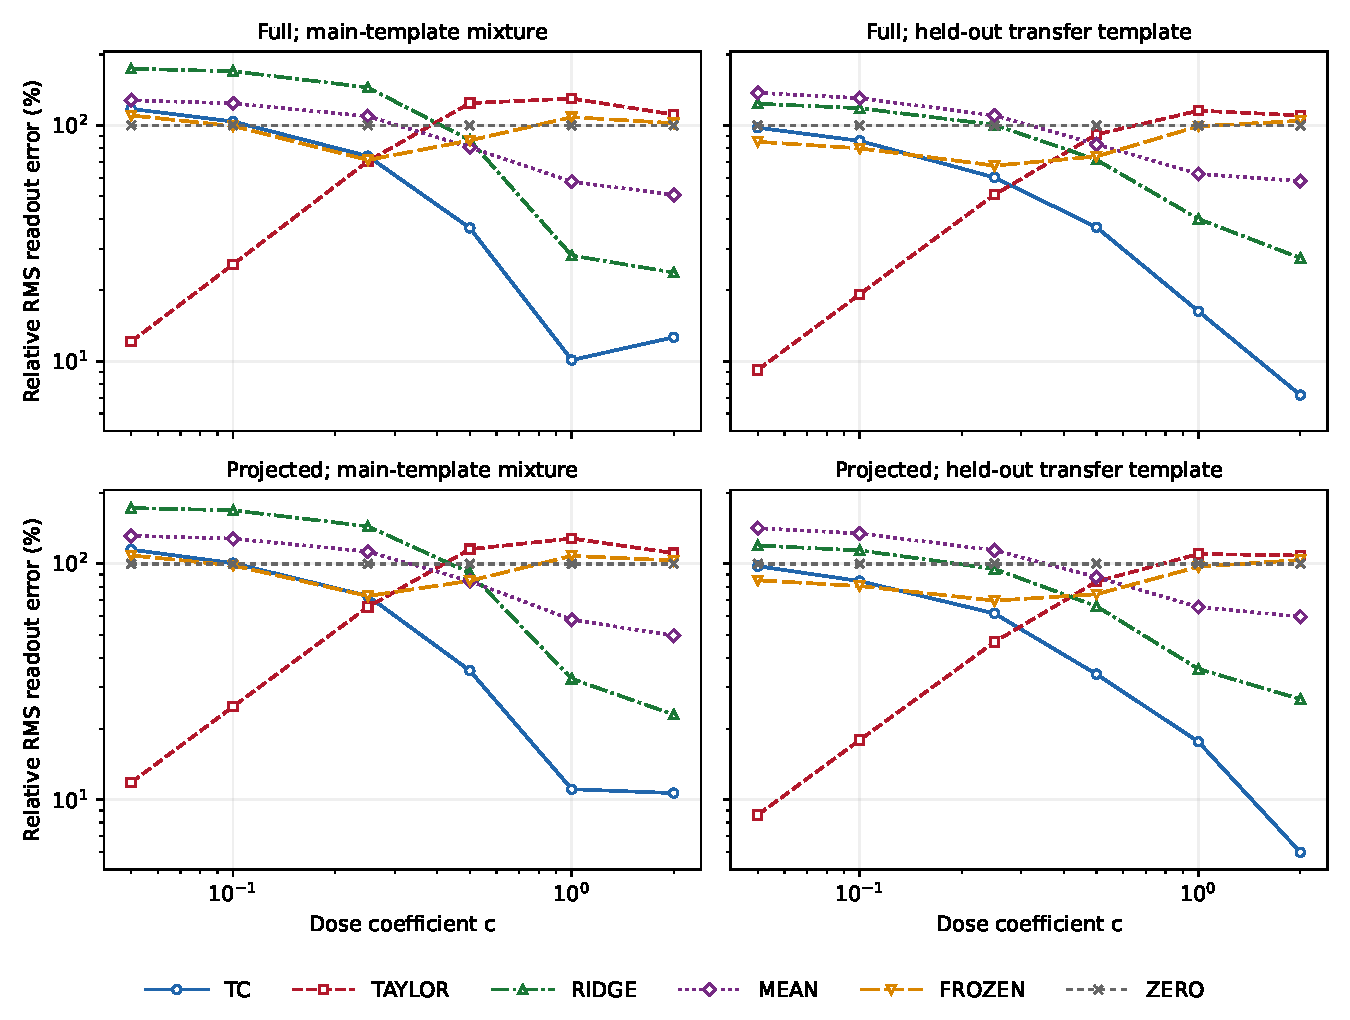
\includegraphics[width=\linewidth]{figures/new_test_dose.pdf}
\caption{All six Gemma-270M TEST doses, main mixture and transfer; pooled relative RMS error. Full numerical grids are in the supplement.}\label{fig:dose}
\end{figure}

\subsection{Gemma-1B: the crossover repeats, the accuracy does not}\label{sec:second}
The second artifact repeats Taylor's small-dose advantage and large-dose failure, but at the full patch its transcoder error, 115.38\% (nominal interval [112.72\%, 118.25\%]), exceeds zero change, ridge and the class mean (Table~\ref{tab:second}). In absolute terms it is .4406 logits against a native signal of .3819. At dose 2 it beats zero change and the mean, but not ridge. Crossover and useful accuracy are therefore empirically separable: a replacement can dominate a poor local approximation without predicting the intervention well.

\begin{table}[ht]\centering\small
\begin{tabular}{lrrrrr}\toprule Condition & TC & Taylor & Ridge & Mean & Zero\\\midrule
Main, $c=.05$ & 134.18 & 23.56 & 84.78 & 94.91 & 100\\
Main, $c=1$ & 115.38 & 269.86 & 50.80 & 66.99 & 100\\
Main, $c=2$ & 41.86 & 110.86 & 34.63 & 43.73 & 100\\
Transfer, $c=1$ & 137.43 & 267.26 & 60.81 & 74.98 & 100\\\bottomrule\end{tabular}
\caption{Gemma-1B relative RMS error, percent, on 256 further blocks. All 144 cells are in the supplement.}\label{tab:second}
\end{table}

\begin{figure}[ht]\centering
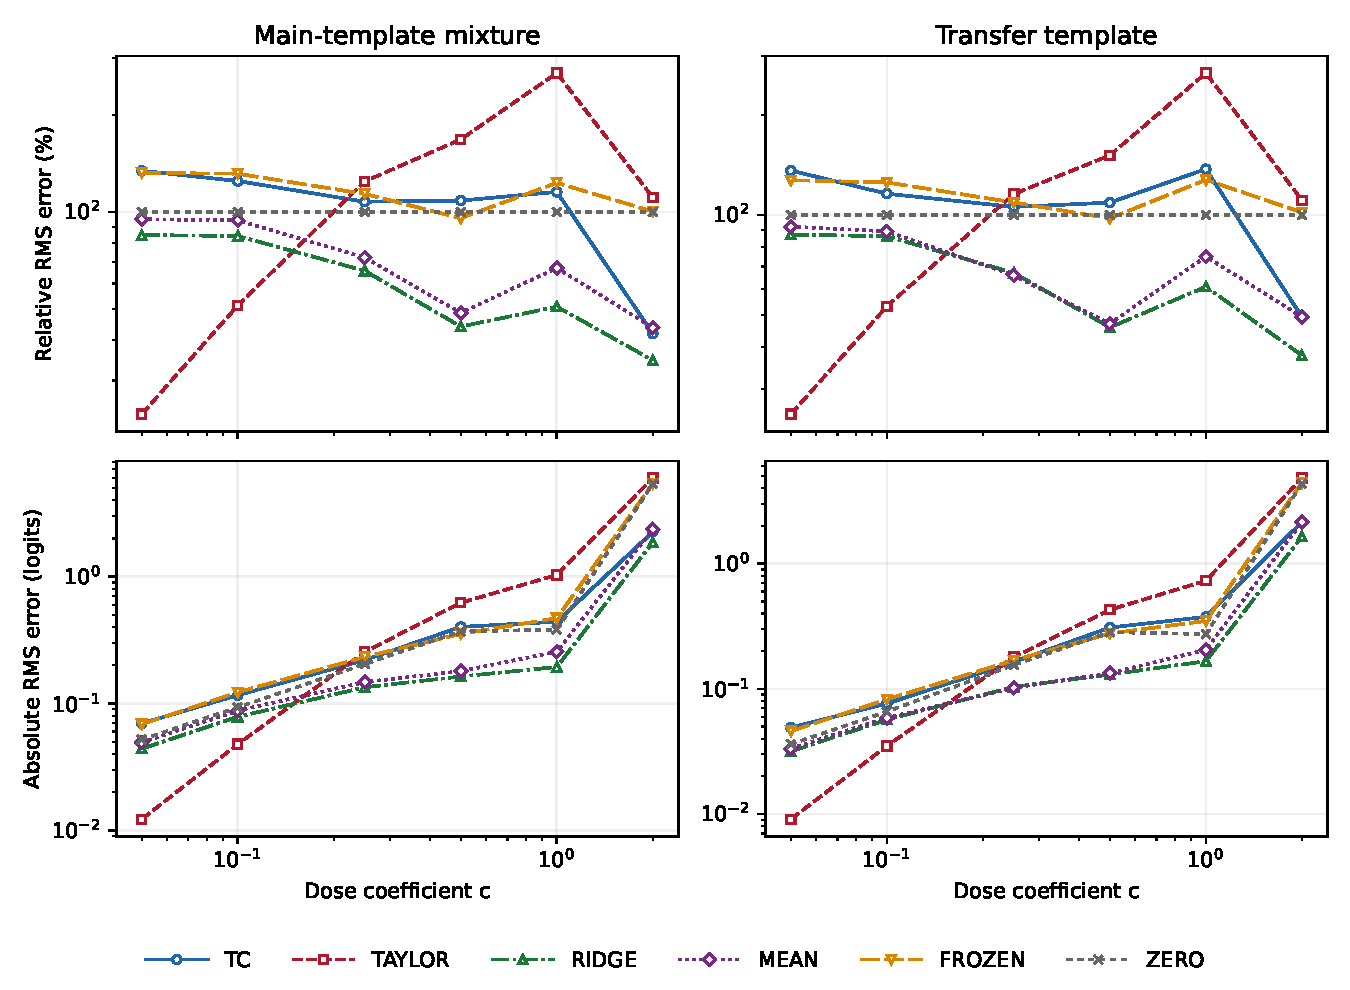
\includegraphics[width=\linewidth]{figures/second_artifact_dose.pdf}
\caption{Second-artifact dose curve. Relative and absolute rankings agree within each condition.}\label{fig:second}
\end{figure}

\section{What the first artifact's error looks like}
\subsection{Endpoint cancellation}
With endpoint reconstruction errors $e_0=T(z)-f(z)$ and $e_1=T(z+\delta)-f(z+\delta)$, the predicted delta error is $e_1-e_0$, with energy $\mathbb E\|e_1\|^2+\mathbb E\|e_0\|^2-2\mathbb E(e_1^\top e_0)$. At the full patch each endpoint carries energy $1.36\times10^6$, yet the delta error carries only $.71\times10^6$: most reconstruction error is shared between endpoints and cancels. The cancelling part is largely a mean offset; centered within each template the cross term is slightly positive. Cancellation shrinks the vector error, but the vector residual still grows with dose (RMS 95.3 at $c=.05$ to 840.6 at $c=1$), so the readout result also depends on how the native suffix filters that residual: at $c=1$ the natural-point gradient term has RMS .267 logits against an observed readout-error RMS of .345, with a nonlinear remainder of RMS .127.

\subsection{Residual direction and decisive threshold switches}
On 32 previously observed blocks (768 conditions), replacing each full-dose residual with a partner residual of the same norm (cyclic shifts 1 and 7) increases readout MSE from .11153 to .14940/.18659 for full edits and from .12119 to .23641/.25200 for projected edits; every full-dose frame favors the original direction. The transcoder's residual is thus oriented favorably for this readout, not merely small.

A mask decomposition shows where the large-dose response is carried. Writing the endpoint code as a base term with the baseline mask plus the contribution of features that switch, we either keep only the switches of 32 FIT-selected features (ONLY) or all switches except theirs (EXCEPT). At full dose, ONLY gives MSE .10463, essentially the original .11153, while EXCEPT gives 8.93294 (projected: .11782 and 7.45841 versus .12119). About eight threshold crossings per context carry the transcoder's full-patch accuracy. Random 32-feature groups rarely switch at all (no switches in 188/192 contexts), so they are not a strength-matched control.

To compare directions at equal strength, we rescale each group's summed switch contribution to a fixed norm, $y_G=y_{\mathrm{TC\_FULL}}-\rho S_G/\|S_G\|$, with groups and $\rho$ fixed on FIT. Removing the top32 direction damages prediction far more than removing five alternative directions (Table~\ref{tab:norm}), on observed and on 32 fresh lexical blocks. The alternatives overlap (one to four distinct directions per context), and top32 was selected by its contribution to the transcoder prediction, so this contrast shows that the prediction's accuracy is concentrated in those switches; it does not identify a native circuit. A control along the transcoder's own predicted delta and a gradient at TC\_FULL would separate prediction-alignment from readout sensitivity; the MSE increment decomposes exactly as $(\Delta m)^2+2e\Delta m$, so both matter.

\begin{table}[ht]\centering\small
\begin{tabular}{lrrr}\toprule Cohort/frame & Eligible contexts & Blocks & Top minus controls\\\midrule
Observed so/when & 128/128 & 32/32 & .165807\\
Fresh lexical so/when & 128/128 & 32/32 & .198352\\
Fresh changed context & 45/64 & 26/32 & .083652\\
Fresh object/readout & 12/64 & 9/32 & .013883\\\bottomrule\end{tabular}
\caption{Full-dose fixed-norm direction diagnostic, squared-logit MSE increment; positive means more damage from removing the top32 direction. Descriptive; coverage requires eligibility of all six groups.}\label{tab:norm}
\end{table}

\section{A negative boundary: a Qwen CLT component}
The public Qwen3-0.6B-Base cross-layer transcoder component from source layer 27 to target layer 27, evaluated through the final norm and head for is/are on 256 blocks shared with the companion study, stays at the zero-change baseline at every dose (Table~\ref{tab:qwen}): at full dose its absolute error is 2.455 logits against a native signal of 2.447, while Taylor has .847 and ridge .748. The operator passed hook, head, JVP and reachability checks. The Gemma-like favorable regime is thus not a generic property of public replacement artifacts; model, layer, readout and artifact type all differ, so the contrast does not isolate a cause.

\begin{table}[ht]\centering\small
\begin{tabular}{lrr}\toprule Predictor & $c=.05$ & $c=1$\\\midrule
CLT component & 99.830 & 100.347\\
Native-vector Taylor & 3.172 & 34.600\\
Composed scalar linear & 3.305 & 35.904\\
Frozen recipient mask & 99.830 & 100.302\\
FIT ridge & 36.499 & 30.572\\
FIT conditional mean & 37.589 & 37.757\\
Zero change & 100.000 & 100.000\\\bottomrule\end{tabular}
\caption{Qwen component relative RMS error, percent, T2/T5 mixture.}\label{tab:qwen}
\end{table}

\section{Discussion}
Local fidelity, ranking against local linearization and finite-effect accuracy are three different properties of a replacement model, and they came apart in every artifact we tested. The Gemma-270M transcoder is a poor local model yet predicts full-patch effects to about 10\%, better than a ridge map trained on native vector changes; the Gemma-1B transcoder shows the same crossover without that accuracy; the Qwen CLT component shows neither. For anyone using a transcoder to predict or choose interventions, the practical consequence is that fidelity should be measured at the intervention size of interest, against strong baselines, rather than inferred from reconstruction, Jacobians or superiority to Taylor.

The scope is one selected public artifact with a clear positive result, one replication of the crossover, synthetic pronoun contexts and two-token readouts. Within that scope the first artifact's success is linked to cancelling endpoint errors, a favorably oriented residual and a few decisive threshold switches; a predictive account of which artifacts reach this regime remains open. Complete dose grids, earlier hypotheses and failed forecasts, operation accounting and independent reviews are in the supplement. Authorship, evidence location and release disclosures remain to be completed.

\clearpage
\small
\bibliographystyle{plain}
\bibliography{references}
\end{document}
